The Harlan J.~Smith Book Collection at the McDonald Library
numbers over 500 items with ??? catalogued entries.

The first books were sent to the McDonald library in ????  I began
cataloguing them on 1 Dec 2021 and finally finished the collection on
23 Oct 2022 after a long delay. There are 298 catalogued items in the
original collection at McDonald though some of the catalogue entries
contain multiple reprints and articles.

A second set of 4 boxes sent on 2 November 2021.  I took them home on
10 April 2022 and finished cataloguing them on 11 April 2022. There
were 4 boxes and 57 items in this second shipment. A third set of
books was received on 29 March 2022. These were catalogued on 9--10 April
2022. There were three boxes and 94 items in the third
shipment. Jeffery Mallon mailed these boxes to me. Finally, a fourth
shipment was received on 13 April 2022 and catalogued on 16--17 April
2022. There were two boxes (1 cu ft) and 1 small box (1/2 cu ft)
containing 54 items in the fourth collection.

Many of the items contain a bookplate ``From the library of Harlan
J.~Smith''.  This bookplate as designed by Joan Smith and added when
the books were first sent to the McDonald Library. The plate shows
Mt.~Locke as viewed from the east with the Harlan J.~Smith telescope
in the foreground, the 82 inch Otto Struve telescope behind it, and
the 36 inch telescope to the left.The Latin inscription ``Sic itur ad
astra'' translates as ``So we go to the stars''. See the figure on the
next page.

Many of the books contain the library stamp of Harlan J.~Smith usually
on the title page.  This stamp was added by Harlan.

A number of books appear to have been purchased from used book dealers.
There are also a number of duplicate books to be found among all the
entries.

Harlan's interests, as indicated by books, are primarily in planetary
studies and space exploration/development. But there are also works on
the history of astronomy, philosophy of science, life on earth, and the
colonization of space. There is also a strong interest in climate
change dating back to the 1970's.

The catalogue is sorted by year and author. The HJS catalogue number
is ``HJS Shipment\#.Box\#.count'' and basicly indicates the order in
which the items were added to the catalogue. The catalogue entry
format is,
\newline

\footnotesize{index} Author/Editors, {\bf Title}

year, Place, Publisher\hspace{1em}pagination

edition if known

series name if a part of a published series

publishing comments

comments about the condition of the item

ownership marks of HJS

HJS catalogue number
\clearpage
% need need photo with less bluring
\begin{figure}
  \centering
  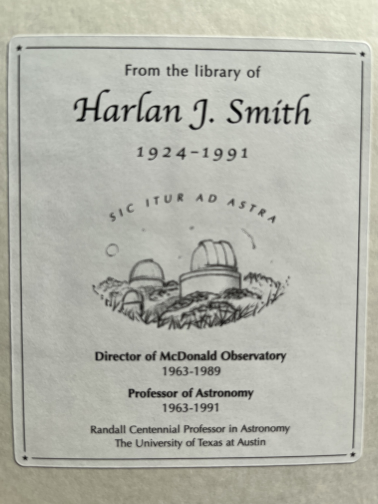
\includegraphics{hjs_bookplate_small.png}
  
  Bookplate of the HJS library. Designed by Joan Smith.
  \label{fig:bookplate}
\end{figure}


